\documentclass[12pt]{article}
\usepackage[english,ukrainian]{babel}
\usepackage[letterpaper,top=2cm,bottom=2cm,left=3cm,right=3cm,marginparwidth=1.75cm]{geometry}
\usepackage{amsmath}
\usepackage{graphicx}
\usepackage{booktabs}
\usepackage{listings}
\usepackage{xcolor}
\usepackage[utf8]{inputenc}
\usepackage{multirow}

\definecolor{codegreen}{rgb}{0,0.6,0}
\definecolor{codegray}{rgb}{0.5,0.5,0.5}
\definecolor{codepurple}{rgb}{0.58,0,0.82}
\definecolor{backcolour}{rgb}{0.95,0.95,0.92}

\lstdefinestyle{mystyle}{
    backgroundcolor=\color{backcolour},   
    commentstyle=\color{codegreen},
    keywordstyle=\color{magenta},
    numberstyle=\tiny\color{codegray},
    stringstyle=\color{codepurple},
    basicstyle=\footnotesize\ttfamily,
    breakatwhitespace=false,         
    breaklines=true,                 
    captionpos=b,                    
    keepspaces=true,                 
    numbers=left,                    
    numbersep=5pt,                  
    showspaces=false,                
    showstringspaces=false,
    showtabs=false,                  
    tabsize=2
}

\lstset{style=mystyle}
\usepackage[colorlinks=true, allcolors=blue]{hyperref}
\usepackage{pgfplots}
\pgfplotsset{compat=1.17}

\title{\textbf{Експериментальна оцінка ентропії на символ джерела відкритого тексту}}
\author{}
\date{}

\begin{document}
\maketitle
\section{Мета роботи}
\quad Засвоєння понять ентропії на символ джерела та його надлишковості, вивчення та порівняння різних моделей джерела відкритого тексту для наближеного визначення ентропії, набуття практичних навичок щодо оцінки ентропії на символ джерела.

\section{Хід роботи}
\quad Для виконання поставленого завдання, після короткого аналізу, я вирішив розбити його на три різних частини: 
\begin{itemize}
    \item робота з файлами та вхідним текстом
    \item робота з літерами
    \item робота з біграмами
\end{itemize}

\subsection{Робота з файлами та вхідним текстом}
\quad Не буду вдаватись в деталі реалізації, так як це не є настільки важливим в даній роботі, лише хочу зазначити, що вхідний текст має назву \texttt{boloto.txt}, цей же текст, але вже опрацьований препроцесором має назву \texttt{boloto\_processed.txt}, а вже оброблений файл та ще й без пробілів має назву \texttt{boloto\_without\_spaces.txt}.

\subsection{Робота з літерами}
\quad В даній секції ми розв'язуємо декілька задач:
\begin{itemize}
    \item підрахунок загальної к-ті літер у тексті
\begin{lstlisting}[language=Rust]
fn letters_count(letter_frequencies: &HashMap<char, i64>) -> i64 {
    let mut count = 0;
    for (_key, _value) in letter_frequencies {
        count += _value;
    }
    count
}
\end{lstlisting}

    \item підрахунок к-ті кожної літери
\begin{lstlisting}[language=Rust]
fn get_letter_frequency(text: &str) -> HashMap<char, i64> {
    let mut frequencies: HashMap<char, i64> = HashMap::new();

    for c in text.chars() {
        *frequencies.entry(c).or_insert(0) += 1;
    }

    frequencies
}
\end{lstlisting}
    \item підрахунок ймовірності зустірти кожну окрему літеру
\begin{lstlisting}[language=Rust]
fn count_letters_probabilities(letter_frequencies: &HashMap<char, i64>) -> HashMap<char, f64> {
    let mut probabilities: HashMap<char, f64> = HashMap::new();
    let number_of_characters = letters_count(letter_frequencies) as f64;

    for (_key, _value) in letter_frequencies {
        probabilities.insert(*_key, (*_value as f64) / number_of_characters);
    }
    probabilities
}
\end{lstlisting}

    \item вивід знайдених значень
\begin{lstlisting}[language=Rust]
fn print_letters_probabilities(probabilities: &HashMap<char, f64>) {
    let mut sorted_probabilities: Vec<(&char, &f64)> = probabilities.iter().collect();
    sorted_probabilities.sort_by(|a, b| b.1.partial_cmp(a.1).unwrap());
    for (&letter, &probability) in sorted_probabilities {
        println!("{}: {}", letter, probability);
    }
    println!();
}

fn print_letter_frequencies(letter_frequencies: &HashMap<char, i64>) {
    let mut sorted_frequencies: Vec<(&char, &i64)> = letter_frequencies.iter().collect();
    sorted_frequencies.sort_by_key(|&(_, frequency)| *frequency);
    for (&letter, &frequency) in sorted_frequencies.iter().rev() {
        println!("{}: {}", letter, frequency);
    }
    println!();
}
\end{lstlisting}
\end{itemize}

\subsection{Робота з біграмами}
\quad Аналогічні задачі доводиться розв'язувати і у випадку з біграмами, правда реалізація буде досить сильно відрізнятись.
\begin{itemize}
    \item підрахунок загальної к-ті біграм у тексті
\begin{lstlisting}[language=Rust]
fn bigram_count(bigram_frequencies: &HashMap<String, i64>) -> i64 {
    let mut count = 0;
    for (_key, _value) in bigram_frequencies {
        count += _value;
    }
    count
}
\end{lstlisting}

    \item підрахунок к-ті кожної з біграм
\begin{lstlisting}[language=Rust]
fn get_bigram_frequency(text: &str) -> HashMap<String, i64> {
    let mut frequencies: HashMap<String, i64> = HashMap::new();

    let mut chars = text.chars().peekable();
    while let (Some(curr), Some(&next)) = (chars.next(), chars.peek()) {
        if curr.is_alphabetic() && next.is_alphabetic() {
            let bigram = format!("{}{}", curr.to_lowercase(), next.to_lowercase());
            *frequencies.entry(bigram).or_insert(0) += 1;
        } else if curr.is_alphabetic() && next.is_whitespace() {
            let bigram = format!("{} ", curr.to_lowercase());
            *frequencies.entry(bigram).or_insert(0) += 1;
        } else if curr.is_whitespace() && next.is_alphabetic() {
            let bigram = format!(" {}", next.to_lowercase());
            *frequencies.entry(bigram).or_insert(0) += 1;
        }
    }
    frequencies
}
\end{lstlisting}
    \item підрахунок ймовірності зустірти кожну окрему біграму
\begin{lstlisting}[language=Rust]
fn count_bigram_probabilities(bigram_frequencies: &HashMap<String, i64>) -> HashMap<String, f64> {
    let mut probabilities: HashMap<String, f64> = HashMap::new();
    let number_of_bigrams = bigram_count(bigram_frequencies) as f64;

    for (_key, _value) in bigram_frequencies {
        probabilities.insert(_key.clone(), (*_value as f64) / number_of_bigrams);
    }

    probabilities
}
\end{lstlisting}

    \item вивід знайдених значень
\end{itemize}


\newpage
\section{Результати роботи}
\subsection{Текст з пробілами}
\subsubsection{Робота з літерами}
\begin{table}[htbp]
\centering
\begin{tabular}{|c|c|c|}
\hline
Літера & Кількість & Ймовірність \\ \hline
' ' & 248583 & 0.0149 \\
а & 115586 & 0.06929 \\
б & 23656 & 0.01418 \\
в & 65348 & 0.03918 \\
г & 23164 & 0.01389 \\
д & 43783 & 0.02625 \\
е & 113939 & 0.06831 \\
ё & 2136 & 0.00128 \\
ж & 12555 & 0.00753 \\
з & 21398 & 0.01283 \\
и & 107358 & 0.06436 \\
й & 17005 & 0.01019 \\
к & 47901 & 0.02872 \\
л & 56102 & 0.03363 \\
м & 46423 & 0.02783 \\
н & 92312 & 0.05534 \\
о & 158172 & 0.09482 \\
п & 41612 & 0.02495 \\
р & 67768 & 0.04063 \\
с & 77815 & 0.04665 \\
т & 96940 & 0.05811 \\
у & 37574 & 0.02253 \\
ф & 4406 & 0.00264 \\
х & 11742 & 0.00704 \\
ц & 6460 & 0.00387 \\
ч & 20695 & 0.01241 \\
ш & 9662 & 0.00579 \\
щ & 4685 & 0.00281 \\
ы & 25661 & 0.01538 \\
ь & 24874 & 0.01491 \\
э & 6029 & 0.00361 \\
ю & 10427 & 0.00625 \\
я & 25800 & 0.01547 \\
ъ & 513 & 0.00031 \\ \hline
\end{tabular}
\label{tab:letter-results}
\end{table}

\newpage
\subsubsection{Робота з біграмами}
\begin{figure}[htbp]
    \centering
    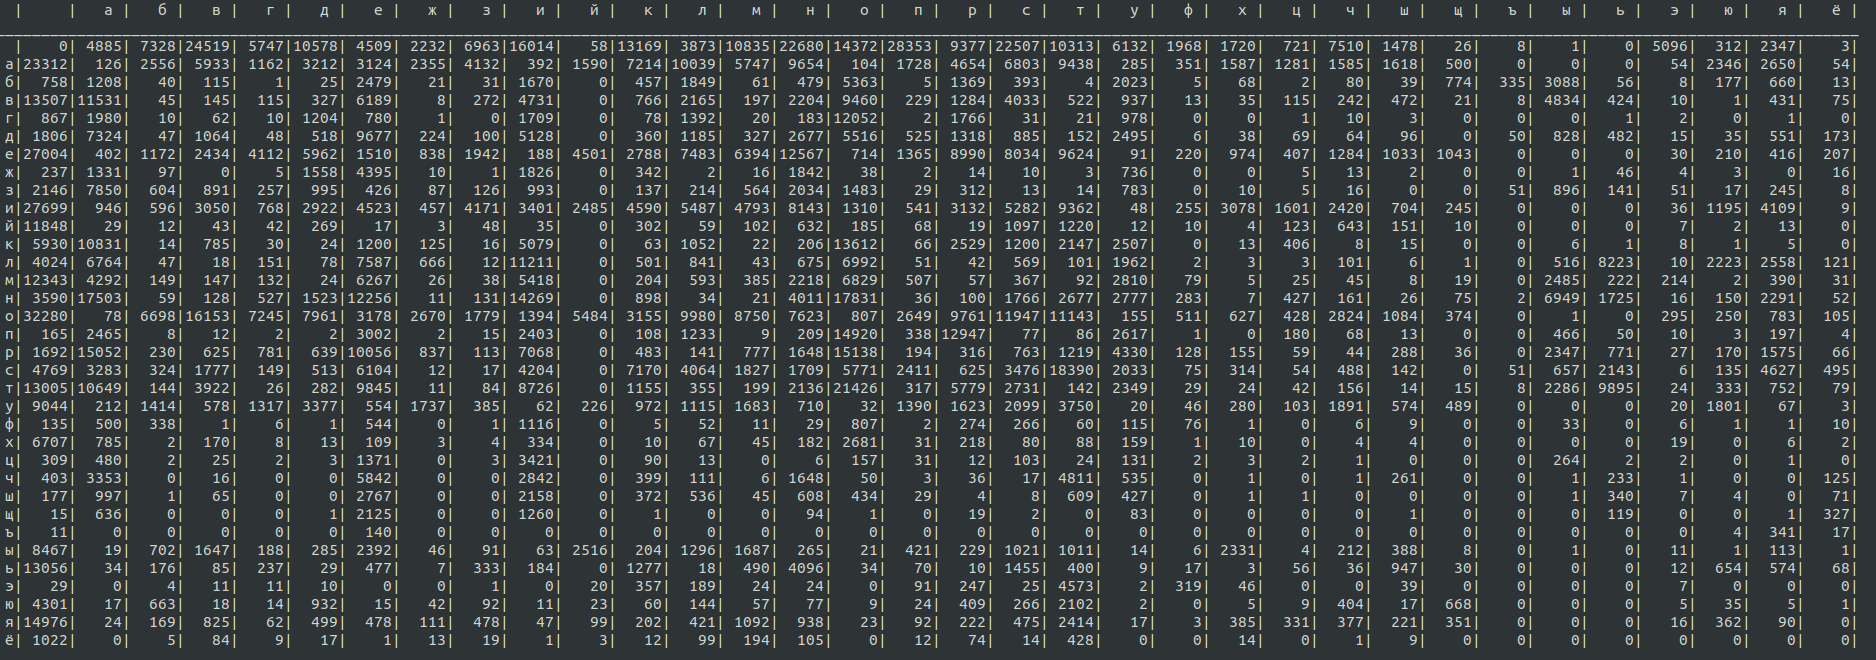
\includegraphics[width=1.0\textwidth]{screenshots/bigram_freq_with_space.png}
    \caption{к-ть біграм}
    \label{fig:screenshot}
\end{figure}
\begin{figure}[htbp]
    \centering
    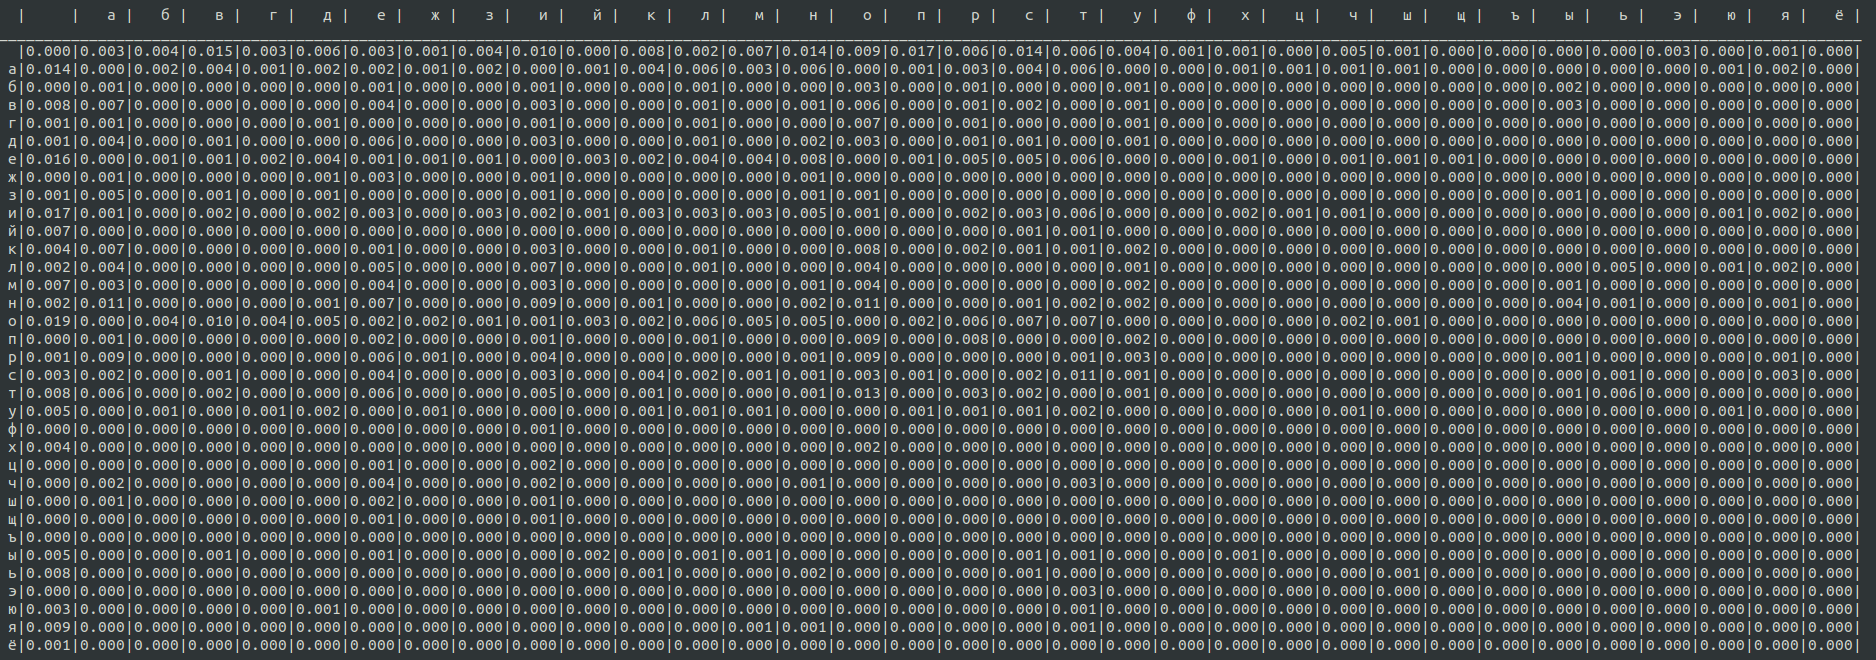
\includegraphics[width=1.0\textwidth]{screenshots/bigram_prob_with_space.png}
    \caption{ймовірність появи біграм}
    \label{fig:screenshot}
\end{figure}

\newpage
\subsection{Текст без пробілів}
\subsubsection{Робота з літерами}
\begin{table}[htbp]
\centering
\begin{tabular}{|c|c|c|}
\hline
Літера & Кількість & Ймовірність \\ \hline
а & 115586 & 0.08143 \\
б & 23656 & 0.01667 \\
в & 65348 & 0.04604 \\
г & 23164 & 0.01632 \\
д & 43783 & 0.03084 \\
е & 113939 & 0.08027 \\
ё & 2136 & 0.00150 \\
ж & 12555 & 0.00884 \\
з & 21398 & 0.01507 \\
и & 107358 & 0.07563 \\
й & 17005 & 0.012 \\
к & 47901 & 0.03374 \\
л & 56102 & 0.03952 \\
м & 46423 & 0.0327 \\
н & 92312 & 0.06503 \\
о & 158172 & 0.11143 \\
п & 41612 & 0.02931 \\
р & 67768 & 0.04774 \\
с & 77815 & 0.05482 \\
т & 96940 & 0.06829 \\
у & 37574 & 0.02647 \\
ф & 4406 & 0.0031 \\
х & 11742 & 0.00827 \\
ц & 6460 & 0.00455 \\
ч & 20695 & 0.01458 \\
ш & 9662 & 0.00681 \\
щ & 4685 & 0.0033 \\
ы & 25661 & 0.01808 \\
ь & 24874 & 0.01752 \\
э & 6029 & 0.00425 \\
ю & 10427 & 0.00735 \\
я & 25800 & 0.01818 \\
ъ & 513 & 0.00036 \\ \hline
\end{tabular}
\label{tab:letter-results}
\end{table}

\newpage
\subsubsection{Робота з біграмами}
\begin{figure}[htbp]
    \centering
    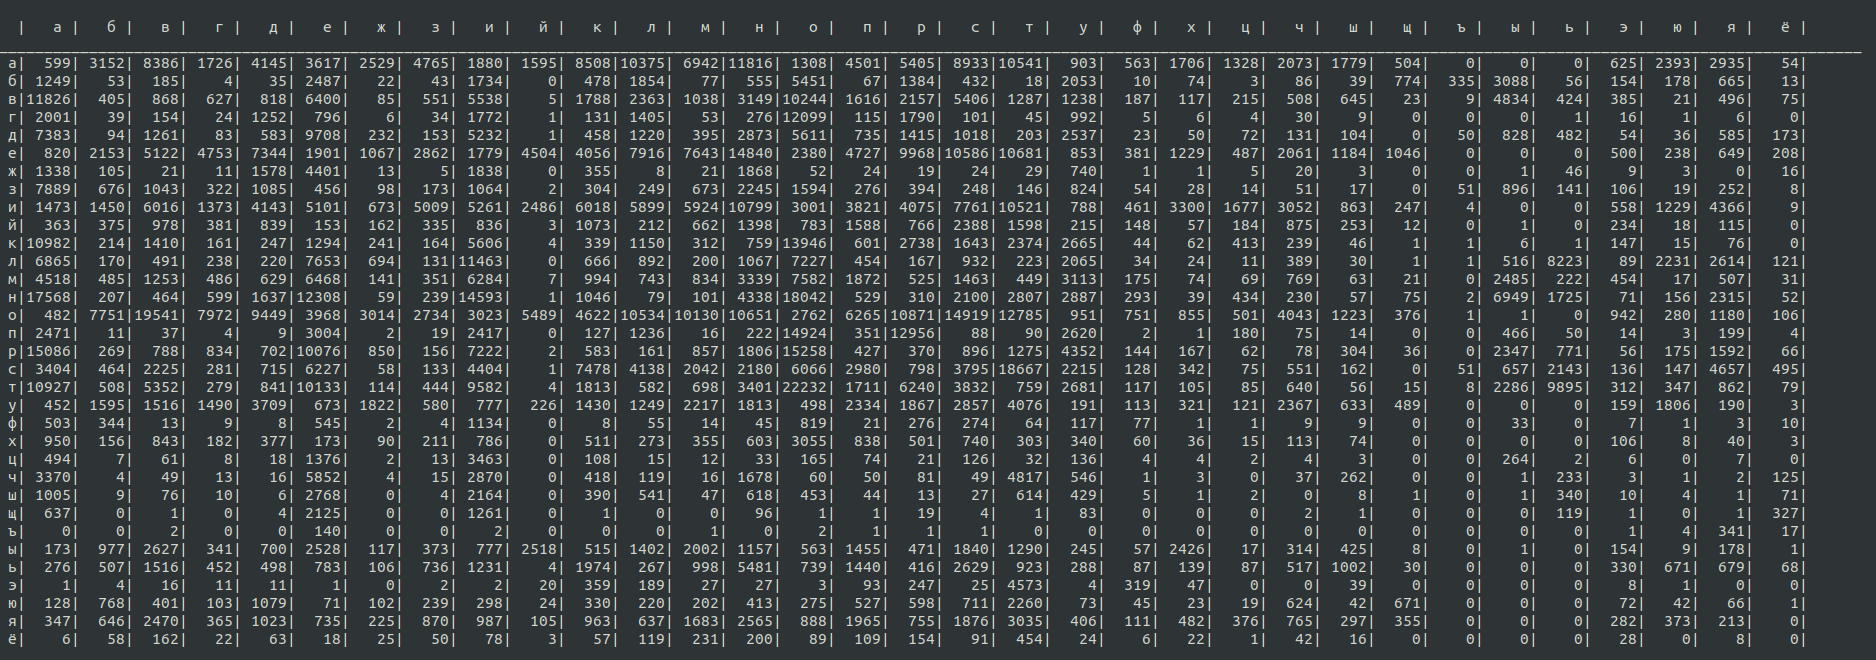
\includegraphics[width=1.0\textwidth]{screenshots/bigram_freq_without_space.png}
    \caption{к-ть біграм}
    \label{fig:screenshot}
\end{figure}
\begin{figure}[htbp]
    \centering
    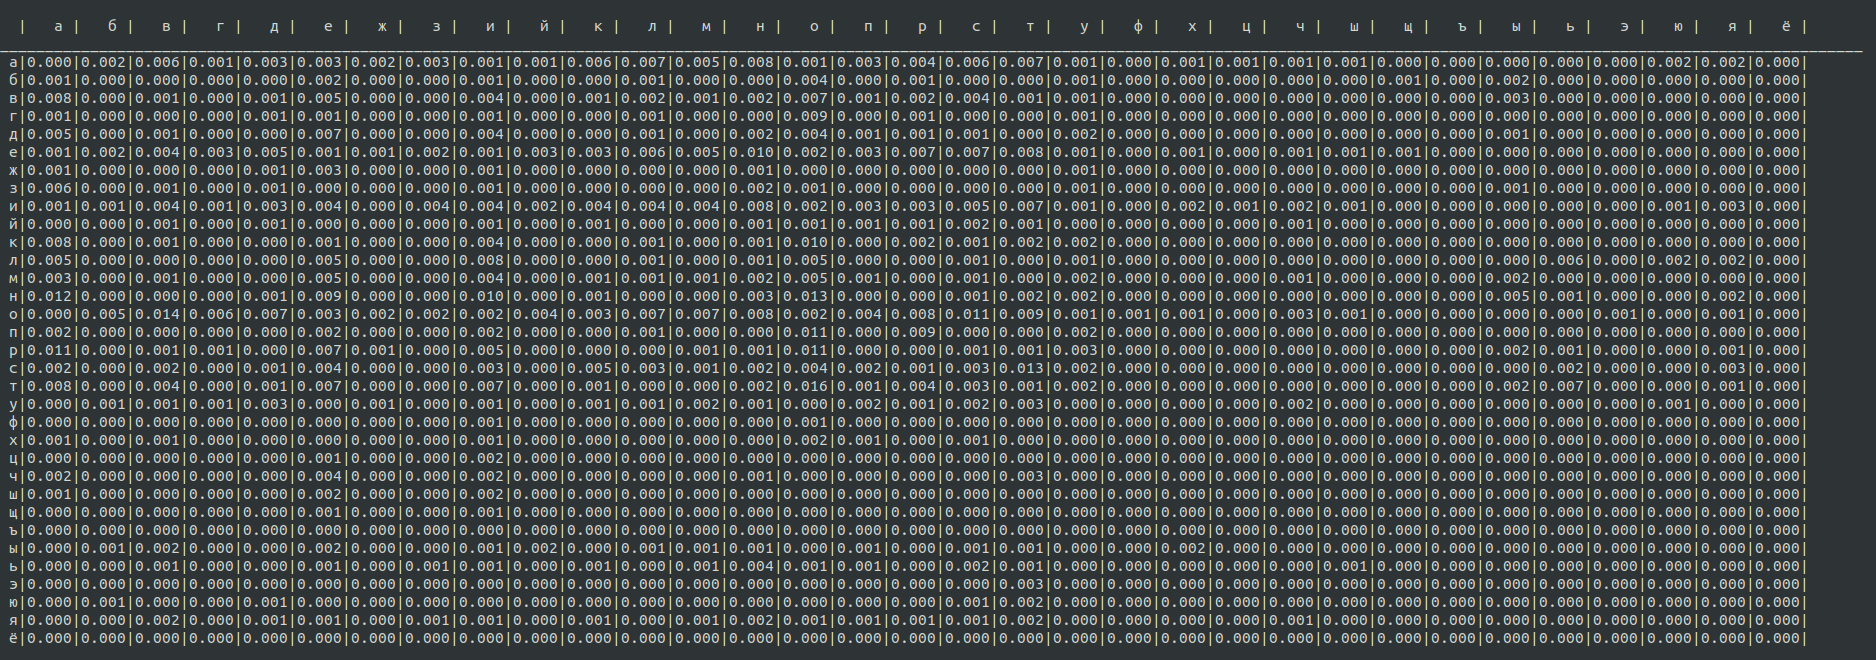
\includegraphics[width=1.0\textwidth]{screenshots/bigram_prob_without_space.png}
    \caption{ймовірність появи біграм}
    \label{fig:screenshot}
\end{figure}

\section{Обчислення ентропій \(H_1\) та \(H_2\)}
\begin{itemize}
    \item Обчислення \(H_1\):
\begin{lstlisting}[language=Rust]
fn compute_h1(letter_frequencies: &HashMap<char, i64>) -> f64 {
    let mut h1 = 0.0;
    let probabilities = count_letters_probabilities(&letter_frequencies);

    for (_key, _value) in probabilities {
        h1 += _value * f64::log2(_value);
    }

    h1 = -h1;
    h1
}
\end{lstlisting}

\newpage
    \item Обчислення \(H_2\):
\begin{lstlisting}[language=Rust]
fn compute_h2(bigram_frequencies: &HashMap<String, i64>) -> f64 {
    let mut h2 = 0.0;
    let probabilities = count_bigram_probabilities(&bigram_frequencies);

    for (_key, _value) in probabilities {
        h2 += _value * f64::log2(_value);
    }
    h2 = -h2/2.0;
    
    h2
}
\end{lstlisting}
Якщо у тексті наявні пробіли, то \(H_1 = 4.404\), якщо ж їх немає, то \(H_1 = 4.461\). 
Так само й для \(H_2\), з пробілами \(H_2 = 4.021\), без \(H_2 = 4.152\).
\end{itemize}

\newpage
\section{Оціночні значення величин \(H^{(10)}\), \(H^{(20)}\) та \(H^{(30)}\)}
\quad Використовуючи програму CoolPinkProgram.exe визначаємо приблизні значення:
\begin{figure}[htbp]
    \centering
    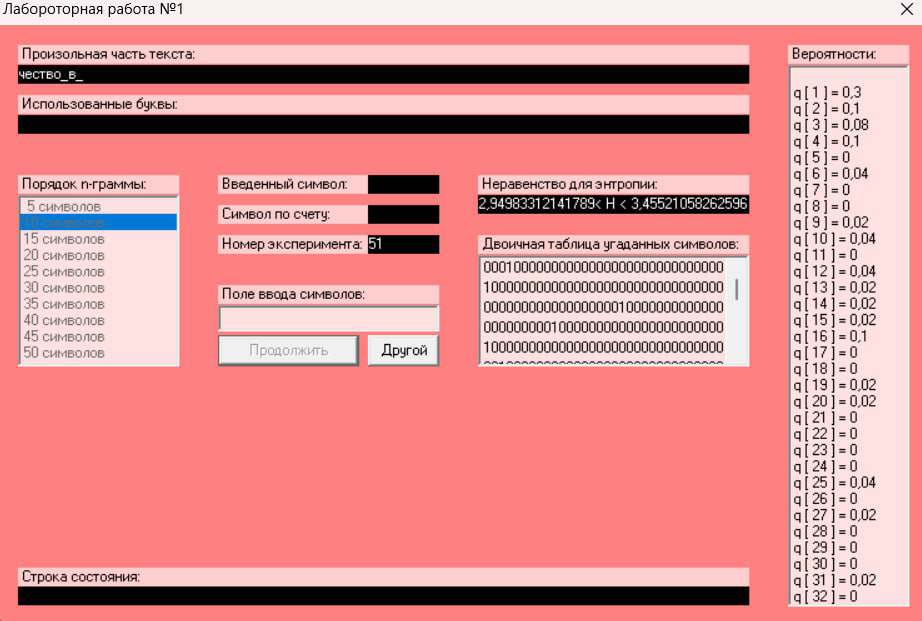
\includegraphics[width=0.75\textwidth]{screenshots/h10.png}
    \caption{значення \(H^{(10)}\)}
    \label{fig:screenshot}
\end{figure}

\begin{figure}[htbp]
    \centering
    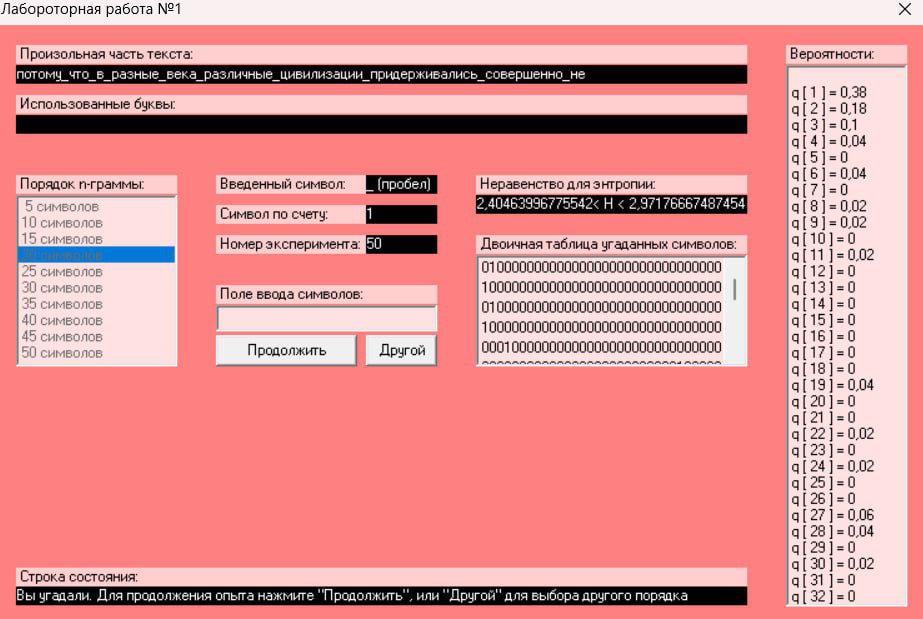
\includegraphics[width=0.75\textwidth]{screenshots/h20.png}
    \caption{значення \(H^{(20)}\)}
    \label{fig:screenshot}
\end{figure}

\begin{figure}[htbp]
    \centering
    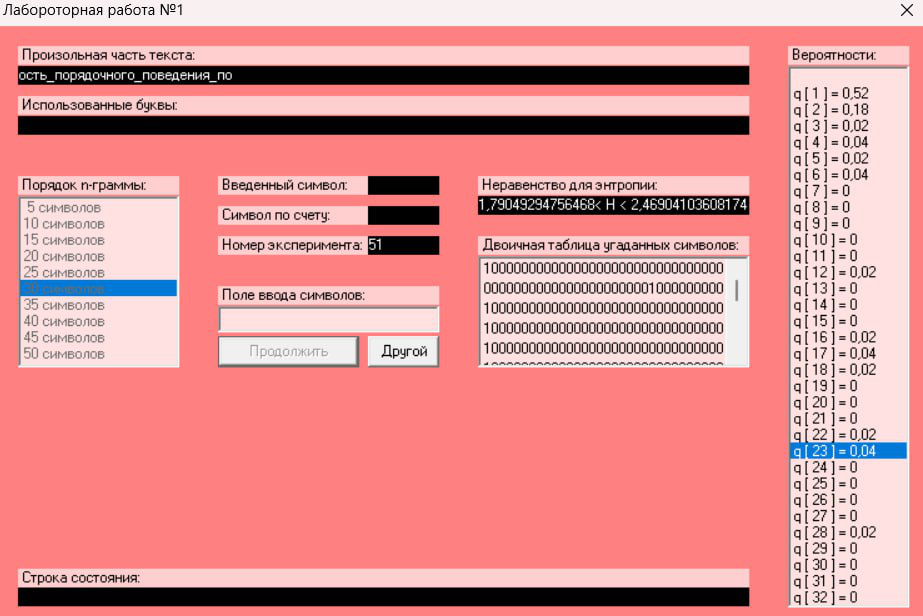
\includegraphics[width=0.75\textwidth]{screenshots/h30.png}
    \caption{значення \(H^{(30)}\)}
    \label{fig:screenshot}
\end{figure}

\newpage
\quad Маємо, що:\\
\begin{center}
$a \leq H^{(10)} \leq c$ \\
$a \leq H^{(20)} \leq c$ \\
$a \leq H^{(30)} \leq c$ \\
\end{center}

Тоді можемо обчислити надлишковість $_{p}$осійської мови \( R \) використовуючи формулу: 

\begin{align*}
R &= 1 - \frac{H_{\text{inf}}}{H_0},
\quad \text{де } H_0 = \log 32 \approx 5 \\
\end{align*}

\begin{center}
$H^{(10)}: 0.4102 \geq R \geq 0.309$ \\
$H^{(20)}: 0.519 \geq R \geq 0.405$ \\
$H^{(30)}: 0.642 \geq R \geq 0.506$ \\
\end{center}

\end{document}